\documentclass[11pt]{article}
\usepackage[hmargin=23mm,vmargin=21mm]{geometry}
\usepackage{amsmath,amssymb,amsthm,booktabs,tikz,hyperref}
\hypersetup{hidelinks}
\newtheorem{theorem}{Theorem}
\newtheorem{proposition}[theorem]{Proposition}
\newtheorem{corollary}[theorem]{Corollary}
\newcommand{\ord}{\operatorname{ord}}
\newcommand{\He}{\operatorname{He}}
\title{Recovering zero multiplicities from subdiscriminants of the backward heat flow}
\author{AI-created mathematical note by GPT-6.2 Astra}
\date{22 November 2026}
\begin{document}
\maketitle
\begin{abstract}
On a fixed contour, the Taylor orders of the subdiscriminants of a backward heat flow determine the complete multiplicity partition of its real endpoint zeros. The partition is read from the first differences of those orders. We derive the leading coefficients and a contour test with an explicit negative-time sign bound. The calculation combines Hermite splitting of a multiple heat zero with the classical Vandermonde formula for subdiscriminants. The zeta application is local in height. Two GPT-6.2 Astra instances derived the order formula, and exact polynomial calculations tested it through degree eight. No human review is recorded.
\end{abstract}

\section{A bounded packet}
Let $H(t,z)$ be jointly holomorphic near $\{0\}\times\overline U$, where $U$ is a bounded conjugation-invariant Jordan domain with piecewise smooth boundary. Assume $H_t=-H_{zz}$, $H(t,\bar z)=\overline{H(t,z)}$ for real $t$, and $H(0,\cdot)$ is nonzero on $\partial U$. Its zeros in $U$ are distinct real centers $c_1,\ldots,c_r$ of respective positive orders $m_1,\ldots,m_r$, of total multiplicity $M$. The argument principle gives the Newton sums
\[
 S_j(t)=\frac1{2\pi i}\oint_{\partial U}z^j
             \frac{H_z(t,z)}{H(t,z)}\,dz,\qquad
 D_k(t)=\det[S_{a+b}(t)]_{0\le a,b<k},\qquad D_0=1 .
\]
They are holomorphic for small complex $t$. Here $S_0=M$, and $D_k$ is the subdiscriminant of order $M-k$ of the monic polynomial of the enclosed zeros.

\begin{theorem}\label{t:orders}
Sort the multiset $\bigsqcup_{i=1}^r\{0,1,\ldots,m_i-1\}$ as $b_1\le\cdots\le b_M$.
Then $\ord_0 D_k=\sum_{j=1}^k b_j$ for $1\le k\le M$. Thus the number of times $h$ occurs among the first differences of these orders equals $\#\{i:m_i\ge h+1\}$. The largest index with $D_k(0)>0$ is $r$.
\end{theorem}

For $H_0(z)=z^3(z-1)$ and $H_0(z)=z^2(z-1)^2$ both full Hankel matrices have rank two at zero time. Their orders distinguish the two endpoint partitions, even if both centers are inside a single contour. Figure~\ref{f:costs} exhibits the integers whose partial sums make this distinction.

\begin{figure}[h]
\centering
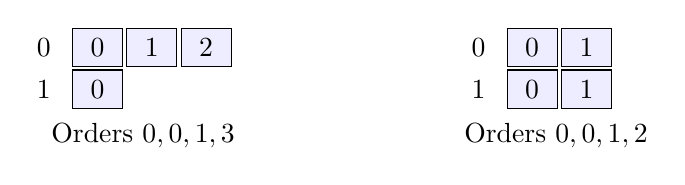
\begin{tikzpicture}[x=0.69cm,y=0.53cm]
\foreach \x/\y/\n in {0/1/0,1/1/1,2/1/2,0/0/0,8/1/0,9/1/1,8/0/0,9/0/1}{
 \draw[fill=blue!7] (\x,\y) rectangle ++(0.92,0.92);
 \node at (\x+.46,\y+.46) {$\n$};}
\node[anchor=east] at (-.22,1.46) {$0$};
\node[anchor=east] at (-.22,.46) {$1$};
\node[anchor=east] at (7.78,1.46) {$0$};
\node[anchor=east] at (7.78,.46) {$1$};
\node at (1.3,-.65) {Orders $0,0,1,3$};
\node at (8.9,-.65) {Orders $0,0,1,2$};
\end{tikzpicture}
\caption{A row corresponds to a center and contains one box per branch. A box counts how many earlier branches from the same center contribute one power of $t$ each to a squared Vandermonde minor. Sorting and summing the cheapest boxes gives Theorem~\ref{t:orders}.}
\label{f:costs}
\end{figure}

\section{The leading terms}
Write $\He_m$ for the monic probabilists' Hermite polynomial and let $h_{m,j}$ be its zeros. At a center $c_i$ the $m_i$ branches obey
\[
 z_{ij}(t)=c_i+\sqrt{2t}\,h_{m_i,j}+O(t).
\]
Indeed put $t=u^2/2$, $z=c_i+uy$ and divide $H(t,z)$ by $u^{m_i}$ and the first nonzero Taylor coefficient in $z-c_i$. The equation $H_t=-H_{zz}$ shows that every monomial of lower weighted order vanishes and the constant term in $u$ is
\[
 \sum_{\ell=0}^{\lfloor m_i/2\rfloor}
   \frac{m_i!(-1)^\ell y^{m_i-2\ell}}{2^\ell\ell!(m_i-2\ell)!}
   =\He_{m_i}(y).
\]
Joint holomorphy gives a convergent expansion on bounded sets of $y$. The Hermite roots are simple and real. The implicit function theorem lifts each root. Constancy of the packet multiplicity accounts for all the roots. At $t>0$ sufficiently small the lifted roots are real.

For integers $0\le a\le m$ define $C(m,0)=1$ and
\[
 C(m,a)=m^a\prod_{\ell=1}^{a-1}(m-\ell)^{a-\ell}\qquad(a\ge1).
\]
Let $v=\sum_{j\le k}b_j$. For each vector of integers $0\le a_i\le m_i$ of sum $k$, write $e(a)=\sum_i\binom{a_i}{2}$.
\begin{proposition}\label{p:leading}
The coefficient of $t^v$ in $D_k(t)$ is
\[
 2^v\sum_{\substack{\sum a_i=k\\ e(a)=v}}
     \prod_i C(m_i,a_i)\prod_{i<j}(c_j-c_i)^{2a_i a_j}.
\]
It is strictly positive.
\end{proposition}
\begin{proof}
Cauchy--Binet expands the Hankel determinant as the sum, over $k$ chosen branches, of the squares of their Vandermonde determinants \cite[Prop.~1]{roy}. For a choice of $a_i$ at center $i$, precisely $e(a)$ squared differences vanish. Each contributes a nonzero positive coefficient times $2t$ on the positive side. Products across centers have the indicated nonzero constant. Choosing the first branch at a center costs zero, the second costs one extra power of $t$, and so on. The cheapest $k$ increments can be taken respecting that order. Thus $\min e(a)=v$. Every minimizing summand has positive leading coefficient. This proves Theorem~\ref{t:orders} and proves the formula with $C(m,a)$ initially expressed as the squared Vandermonde sum on $a$ Hermite roots.

For the closed formula, let $J$ be the symmetric $m$-by-$m$ Jacobi matrix with zero diagonal and successive off-diagonals $\sqrt1,\ldots,\sqrt{m-1}$. The determinant recurrence gives $\det(zI-J)=\He_m(z)$. Cramer's rule at its last vertex gives $\He_{m-1}(z)/\He_m(z)=\He_m'(z)/(m\He_m(z))$. This is the Stieltjes transform of mass $1/m$ at each Hermite root. On reversing the vertex order its monic orthogonal polynomials have recurrence coefficients $m-1,\ldots,1$. In detail, evaluating the degree-$j$ monic polynomial on the reversed matrix at the first basis vector yields a multiple of basis vector $j+1$ equal to the product of the first $j$ off-diagonals. Its squared norm is $\prod_{\ell=1}^j(m-\ell)$. The monic basis change has determinant one. The moment determinant for the counting measure therefore equals the product of these squared norms for $j=0,\ldots,a-1$, multiplied by $m^a$. This is $C(m,a)$.
\end{proof}

\section{The first negative minor}
There is a direct differential formula which avoids following individual branches. Let $Q(z)=\prod_i(z-c_i)$. If any $m_i>1$ then
\[
 D_{r+1}'(0)= 2D_r(0)\sum_i m_i(m_i-1)\,Q'(c_i)^2>0.
 \tag{1}
\]
In fact $D_r(0)=\prod_i m_i\prod_{i<j}(c_j-c_i)^2$. Replace the monomial of degree $r$ in the moment matrix by the monic polynomial $Q$. Its last row and column vanish at $t=0$. Differentiating the determinant leaves only $D_r(0)$ times the derivative of the moment of $Q^2$. For any polynomial $P$, contour integration by parts gives
\[
 \left.\frac{d}{dt}\sum_z P(z)\right|_{t=0}
   =\sum_i\operatorname{Res}_{z=c_i}
     \left[P'(z)\frac{H_{zz}(0,z)}{H(0,z)}\right].
\]
Here the sum on the left runs over the packet with multiplicities. Writing $H(0,z)=(z-c_i)^{m_i}g_i(z)$ yields a double-pole coefficient $m_i(m_i-1)$ and simple-pole coefficient $2m_i g_i'(c_i)/g_i(c_i)$. For $P=Q^2$, $P'(c_i)=0$ and $P''(c_i)=2Q'(c_i)^2$. This proves (1). For a single center of multiplicity $m$ it reads $(m S_2-S_1^2)'(0)=2m^2(m-1)$.

In particular, $D_{r+1}(t)<0$ for all sufficiently small negative $t$ if any center is multiple. If all are simple, $r=M$ and $D_{r+1}$ is identically zero. When an explicit radius is needed, suppose the contour is zero-free for $|t|\le R$ and let $B$ bound $|D_{r+1}(t)|$ on $|t|=R$. If the slope in (1) is $g>0$, Cauchy's estimates bound the remainder by $2B|t|^2/R^2$ for $|t|\le R/2$. The sign is certified for $0<-t<\min(R/2,gR^2/(2B))$.

Two small examples explain the height qualification. For the simple endpoint pair $H(0,z)=z^2-\delta^2$, the minor $D_2(t)=4(\delta^2+2t)$ already turns negative at $t<-\delta^2/2$. A negative observation at one prescribed time can therefore arise from distinct endpoint zeros. For $H(0,z)=z^2(z-\delta)$ one obtains $D_3(t)=8t(\delta^4+18\delta^2t+108t^2)$. A known double zero can have arbitrarily small detecting slope on a contour of fixed size even at total degree three.

\section{Scope for the completed zeta function}
In the normalization of Rodgers and Tao \cite{rt},
$H_0(z)=\tfrac18\xi(\tfrac12+iz/2)$ and $\partial_t H=-H_{zz}$. The preceding argument applies inside any admissible contour containing only real endpoint zeros. It requires neither a simplicity hypothesis nor a bound for the global location of the zeros when reality has been established in that contour. A complex contour with nonreal centers can lose the positivity of the leading Vandermonde terms. The same local statement applies to any real-type completed $L$-function equipped with a jointly holomorphic heat deformation in these coordinates.

At $t=0$ the ordinary trace form counts the distinct centers through its rank. The rank and total alone lose the multiplicity partition. With all the exact endpoint Newton sums available, classical reconstruction already recovers it: the first $M$ sums determine the monic polynomial by Newton's identities, and its square-free decomposition gives the multiplicities. The Taylor orders provide a different, purely integer-valued statistic of the deformation. A global assertion about simplicity would still need control of arbitrarily high packets. In particular $R$, $B$, and the positive slope can all depend on the packet. The contour data here give no uniform control of the global Toeplitz or Jensen detection orders.

\begin{thebibliography}{9}
\bibitem{roy} M.-F. Roy, \emph{Subdiscriminants of symmetric matrices are sums of squares}, Dagstuhl Seminar Proceedings 05021, Proposition 1. \href{https://doi.org/10.4230/DagSemProc.05021.20}{doi:10.4230/DagSemProc.05021.20}.
\bibitem{rt} B. Rodgers and T. Tao, \emph{The de Bruijn--Newman constant is non-negative}, Forum Math. Pi \textbf{8} (2020), e6. \href{https://arxiv.org/abs/1801.05914v5}{arXiv:1801.05914v5}.
\end{thebibliography}
\end{document}
